\documentclass[12pt, git, final]{rureport}


\begin{document} % this tells the compiler that it is time to make
                 % text to print instead of just getting ready.
\maketitle  % make a title page from the Title, Date, and Author

%\fxnote{skoða titil á skýrslu, sbr. forsíðu}

%\section*{Errata} %%section* avoids putting a number 

\section{Inngangur} % sections break up the document into pieces

Í þessu verkefni áttu nemendur að setja fram rannsóknarspurningar sem þeir gætu svarað með gögnum frá Hagstofu Íslands\cite{H}. 
%Fyrst var spurt, hvað er það sem okkur finnst áhugavert, þar sem við allir eru nemendur við Háskóla Reykjavíkur þá fannst okkur tilvalið að fjalla um  menntun og laun ýmissia starfsstétta. 
Ákveðið var að skoða meðaltal heildarlauna eftir starfstétt og kyni.
Spurningin sem sett var fram: Er launamunur á kynjunum?
\\
Eftir að gögnin höfðu verið skoðuð vöknuðu fleiri spurningar.
\begin{itemize} 
	\item Er munur á fjölda vinnustunda karla og kvenna?
	\item Eru meðallaun háð háskólamenntun?
	\item Hvernig skiptist menntunargráða aldurshópa niður á milli ára?
	\item Er munur á kynjahlutfalli þeirra sem sækjast í háskólagráður á höfuðborgarsvæðinu og utan þess?
	\item Hafa laun á vinnumarkaði áhrif á aðsókn í Háskólanám?
\end{itemize}


Gögnin voru þannig að hægt var að svara mörgum spurningum og túlka á margan hátt. Markið var sett á að skoða hvernig menntun og laun dreifðust á milli kynja og út frá þeim gögnum var hægt að spyrja sig að enn fleiri spurningum eins og nefnt er að ofan.

%Í þessu verkefni áttu nemendur að setja fram rannsóknarspurningar sem þeir gætu svarað með gögnum frá Hagstofu Íslands. Fyrst var spurt, hvað er það sem okkur finnst áhugavert, þar sem við allir eru nemendur við Háskóla Reykjavíkur þá fannst okkur tilvalið að fjalla um  menntun og laun ýmissia starfsstétta.// 

%Skoðað var meðaltal heildarlauna starfstétta og eftir þær niðurstöður skoðuðum við meðaltalsvinnustundir á milli kynja milli ára,  hvernig menntunargráða ýmissa aldurshópa skiptist niður á milli ára, skoðum kynjahlutfall háskólagráða innan höfuðborgarsvæðis og utan þess.// 

% Áður en hafist var handa byrjuðum við að setja fram nokkuð opnar spurningar sem snérust að menntun, menntunnar stigum, launum fyrir mismunandi aldurshópa og hvort mætti finna eitthverja fylgni í þessum gögnum.

\section{Framkvæmd}

Gögnin sem voru notuð til að svara spurningunni voru tvær csv skrár. Annars vegar "Laun á almennum vinnumarkaði eftir starfsstétt og kyni 1998-2014"\cite{HG1} og hins vegar "Mannfjöldi eftir menntunarstöðu 2003-2013"\cite{HG2}.

Gögnin voru tekin inn og unnið með þau í Pyhton 3\cite{python3}. Sett voru upp nokkur forrit sem gætu unnið sjálfstætt til að einfalda ferlið, t.d. var eitt forrit sem tók gögnin inn úr csv skránum og skilaði þeim á dictionary formi. Þetta forrit innihélt einnig fall sem prentaði út alla lykla í þessu dictionary til þess að ekki þyrfti að eyða tíma í að lesa hrágögnin og leita að þeim þannig.
Einnig voru gerð forrit sem gátu raðað gildunum í dictionary eftir keys eða values og forrit sem tekur inn lista og breytir gögnunum í listanum í heiltölur. Með þessum verkfærum ásamt Matplotlib\cite{lib} var hægt að vinna með gögnin og teikna gröf á auðveldan máta. 

%Þegar búið var að velja hvaða gögn kæmu til með að vera notuð byrjaði einn hópmeðlimur (K.R.Þ.) að forvinna gögnin í python til að einfalda vinnuna fyrir alla og spara þar með tíma. Inni í þessari forvinnu voru meðal annars búnar til breytur og prentaður út listi með öllum lyklum (keys) í dictionary sem sett var upp. 

%Eftir það settist hópurinn niður og skrifaði spurningar sem okkur fannst áhugaverða og líklegt að það kæmi spennandi niðurstöður úr.

Ferlið sem hrágögnin fara í gegnum er ekki langt. Fyrst eru hrágögnin lesin inn í dictionary, því næst eru viðeigandi gögn síuð út. Þar á eftir er gögnunum raðað og breytt úr strengjum yfir í tölur. Lokaskrefið er þá að teikna upplýsingarnar inn á gröf.

Flóknasti hlutinn kemur til þegar bera á saman gögn úr tveim mismunandi gagnasöfnum á sama grafi, sbr. Mynd \ref{fig:heildarhask} þar sem bæta þurfti við auka y-ás.

Þá tóku allir meðlimir hópsins að sér 1-3 spurningar og skrifuðu kóða fyrir þær. Því næst voru gerð föll fyrir hvern og einn kóða sem skiluðu viðeigandi niðurstöðum og var ein yfirskrá gerð sem birti allar niðurstöðurnar, í þessu tilfelli línu- og súlurit sem birt eru í kafla \ref{nidurstodur} hér að neðan.

%\section{Aðferðir}

%Aðferðafræðin sem var sett á hópfundi, eftir að búið var að forvinna gögin, að allir myndu velja spurningu/ar og vinna úr gögnunum og búa til sinn eigin kóða í Python. Síðan voru gögnin borin saman svo hægt væri að rýna í niðurstöðurnar og svara sem flestum spurningum og hvort væri hægt að draga einhverjar niðurstöður úr þeim niðurstöðum sem fengust.

%Uppbygging kóðanna er mjög svipuð þótt hver og einn gerði sinn eiginn kóða, það er byrjað á því að taka inn allar þær 
 
%Sú aðferðar fræði var tekinn í pólinn að allir í hópnum myndu vinna sinn eiginn kóða, en á 3 tíma fresti væru teknar tíu mínótur


\section{Niðurstöður}\label{nidurstodur}
%vladimir
\subsection{Menntunarstig aldurshópa milli ára}
Á Mynd \ref{fig:menntunall} getum við séð að flestir sem lokið hafa einhverskonar menntun á Íslandi eru á bilinu 30 og 49 ára, næst fjölmennasti aldurshópurinn er 50 til 64 ára.
Áhugavert að skoða hvernig fjöldi menntaðs fólks skiptist á milli kynjanna, menntunnar og aldursflokks. Til dæmis:
\begin{itemize}  
	
	\item Breytingin hjá konum með grunnmenntun árið 2008 þar sem konur í aldursflokki 50 - 64 ára urðu fleiri en þær sem voru 30 - 49 ára eins og sést á Mynd \ref{fig:menntungrunn}.
	
	\item Það eru fleiri konur með háskólamenntun en karlar skv. Mynd \ref{fig:menntunhs}, en það virðist vera vaxandi flokkur hjá konum á aldrinum 30 - 49 ára.
	
	
	\item Það er minna bil á milli aldursflokkanna 30 - 49 og 50 - 69 ára hjá báðum kynjum þegar kemur að starfs- og framhaldsmenntun. Einnig sést að fjöldi kvenna er mjög svipaður á milli aldursflokkanna 20 - 24 og 50 - 64 ára, miðað við karla skv. Mynd \ref{fig:menntunfram}.
	
	\item Einhverja hluta vegna vantar upplýsingar um menntun hjá fleiri körlum en konum skv. Mynd \ref{fig:menntunvantar}.
	
\end{itemize}
%Haukur
Einnig var hlutfall milli karla og kvenna sem öfluðu sér háskólamenntunnar, innan og utan höfuðborgarsvæðisins, skoðað, sbr. Mynd \ref{fig:menntukarla} \& Mynd \ref{fig:menntunkonur}. Við var að búast að konur væru í meiri hluta eftir skimun yfir gögn og eru um 4-6\% sem aðskilja kynin í samanburði á gögnunum. Það sem vakti mikla athygli var að tæplega tvöfalt fleiri karlar sækja sér háskólamenntun innan höfuðborgarsvæðisins en á landsbyggðinni.

%Kristófer
\subsection{Heildarlaun karla og kvenna í mismunandi störfum milli ára}
Þegar heildarlaun karla og kvenna í mismunandi starfsgreinum voru borin saman kom í ljós að í hverri einustu starfsgrein var munur á launum kynjanna: meðaltal heildarlauna karla er alltaf hærra.

Fyrstu gögnin sem voru skoðuð geymdu meðaltal yfir allar starfsgreinar, sbr. línuritið á Mynd \ref{fig:heildarhask}, og þar sést að þegar allt er tekið til greina hafa karlar í dag u.þ.b. 130 þús. kr. hærri mánaðartekjur en konur. Á línuritinu sést líka að karlar virðast vera fleiri á vinnumarkaði þ.s. línan sem sýnir meðaltal milli karla og kvenna liggur nær körlunum.

Þetta kom svo sem ekki mikið á óvart þegar horft er til þess að sjómenn, sem eru ein tekjuhæsta (ef ekki tekjuhæsta) stéttin á Íslandi, eru flestir karlkyns, auk þess sem iðnaðarmenn eru flestir karlkyns. 
Það var því hugsanlegt að þetta myndi skekkja niðurstöðurnar eitthvað.

Því var ákveðið að skoða gögn úr mismunandi starfsstéttum en sama hvaða gögn voru skoðuð, alltaf höfðu mennirnir hærri heildarlaun. Í flestum starfsstéttum virðist kynjahlutfallið vera frekar jafnt, nema í fyrrnefndum greinum. Þegar gögn um fólk í skrifstofustörfum voru skoðuð kom niðurstaðan heldur betur á óvart.

Í skrifstofustörfum eru konur mun fleiri en karlar, sbr. Mynd \ref{fig:heildarlaun}. Þetta sést á því að línan sem táknar meðaltalið liggur eiginlega alveg ofan í línunni sem táknar heildarlaun kvenna. Þrátt fyrir það eru heildarlaun karla u.þ.b. 50 þús. kr. hærri. Þetta kemur á óvart þar sem upp hafði komið kenning um að heildarlaunin skekktust oft á tíðum einfaldlega vegna þess að fleiri einstaklingar í viðkomandi starfsstétt væru karlmenn, svo virðist hins vegar ekki vera raunin.

Að lokum var fjölda einstaklinga sem hafa háskólamenntun bætt inn á Mynd \ref{fig:heildarhask} til að sjá hvort einhver fylgni væri milli heildarlauna og menntunarstigs einstaklinga. Á grafinu má sjá að þetta tvennt virðist haldast nokkuð örugglega í hendur, þó svo að karlarnir virðist eiga erfiðara með að rífa sig upp eftir árið 2008. Samt sem áður eru gögnin ofboðslega lík.

Lokakenningin sem gæti skýrt hvers vegna heildarlaun karla eru hærri en kvenna á einhvern einfaldan og rökréttann hátt var þá að karlar hljóta einfaldlega að vinna meira og fá þ.a.l. hærri laun. Annað kom hins vegar í ljós þegar fjöldi greiddra vinnustunda var skoðaður.

%Róbert
\subsection{Munur á fjölda vinnustunda milli ára}
Þegar skoðaðar voru greiddar stundir (meðaltal yfir árið) á viku fyrir fulla vinnu þá var skoðað hvort mikill munur væri á greiddum vinnustundum á viku milli kynjanna og hvernig það dreifðist yfir árin. 

Það kom í ljós, þegar um var að ræða allar starfsstéttir, að munur á milli karla og kvenna árið 1998 var um 4,2 klukkustundir fyrir greiddar vinnustundir í fullri vinnu en árið 2014 var þessi mismunur kominn niður í um 2,5 greiddar vinnustundir í fullri vinnu.
Það sést á grafinu að mismunurinn minnkar til ársins 2002, eykst svo til ársins 2008 og minnkar loks aftur, sbr. Mynd \ref{fig:unnirtimar1}. Þegar þessi gögn eru borin saman við heildarlaun kynjanna á Mynd \ref{fig:heildarhask} sést að yfir heildina litið fá karlar mun meira borgað en konur, þ.s. greiddar vinnustundir eru svipaðar en mikill munur á heildarlaunum.

Þegar einungis skrifstofustörf voru skoðuð þá sást að munurinn árið 1998 var tæp ein greidd vinnustund. Árið 2014 þá var munurinn svipaður en það var nákvæmlega 1 vinnustund sem skildi kynin að. Þrátt fyrir þetta er meðaltal heildarlaua karla í skrifstofustörfum mun hærra þó svo að konur í skrifstöfustörfum séu fleiri, sbr. Mynd \ref{fig:heildarlaun}. Þróun fjölda vinnustunda var frekar jöfn en munurinn eykst frá árinu 2001  til ársins 2009 og minnkar síðan aftur, sbr. Mynd \ref{fig:unnirtimar1}.

Þegar greiddar vinnustundir á viku voru skoðaðar hjá sérfræðimenntuðu fólki þá er mismunurinn ekki mikill og er hann mestur rúm ein greidd vinnustund milli ára. Árið 2000 þá tóku konurnar fram úr karlmönnunum og fengu fleiri greiddar vinnustundir, en fljótlega eftir 2001 þá tóku karlmennirnir aftur fram úr, sbr. Mynd \ref{fig:unnirtimar2}. Samt sem áður fá karlar enn hærri laun en konur, sbr. Mynd \ref{fig:heildarlaunstjorn}.

Þegar greiddar stundir fyrir stjórnendur voru skoðaðar þá er mismunurinn milli greiddra vinnustunda minna en hálf klukkustund árið 1998. Frá 1999 til 2007 fengu konur fleiri greiddar vinnustundir heldur en karlar. Þegar liðið er á árið 2007 þá fara karlar framúr konum og fá fleiri greiddar vinnustundir en munurinn er innan við ein vinnustund, sbr. Mynd \ref{fig:unnirtimar2}. Þó svo að munurinn á vinnutíma sé þetta lítill eru heildarlaun kvenna í stjórnunarstöðum u.þ.b. 200 þús. kr. lægri en heildarlaun karla sem gegna sömu stöðu árið 2014, sbr. Mynd \ref{fig:heildarlaunstjorn}.

\section{Samantekt}

Samkvæmt gögnum frá Hagstofunni\cite{H} er greinilega launamunur á kynjunum sem nemur að meðaltali um 130 þús. kr. á mánuði, þar sem karlar eru með hærri laun, sbr. Mynd \ref{fig:heildarhask}. Einnig kom í ljós að karlar vinna að meðaltali um 2,5 klst meira á viku en það gæti til dæmis stafað af fæðingarorlofi þar sem konur taka í flestum tilfellum lengri fæðingarorlof, sbr. Mynd \ref{fig:unnirtimar1}. Því virðist nokkuð öruggt að karlar fá almennt meira borgað en konur og munurinn virðist hvorki stafa af því að fleiri karlar vinni í hálaunastörfum né að karlar einfaldlega vinni meira.

Greinilega sést á gögnunum að það aldursbil sem líklegast er að hafa menntun er 30 - 49 ára í öllum tilvikum nema grunnmenntun en það bendir til þess að fleiri ljúka grunnmenntun nú en á árum áður, sbr. Mynd \ref{fig:menntungrunn}. Einnig eru fleiri sem stunda háskólamenntun innan höfuðborgarsvæðisins en utan þess. Þetta stafar líklega af fjölda námsmöguleika sem höfuðborgin hefur fram yfir landsbyggðina, sbr.  Mynd \ref{fig:menntukarla} \& Mynd \ref{fig:menntunkonur}.

Þegar laun á vinnumarkaðinum eru skoðuð ásamt gögnum um háskólamenntun virðist vera einhver tenging þar á milli. Það sést á Mynd \ref{fig:heildarhask} að fjöldi háskólamenntaðra fylgir eftir launum á vinnumarkaði þ.e. súluritið hefur svipaða lögun og línuritið en er hliðrað til hægri. Þetta sýnir að fjöldi fólks með háskólamenntun er háð heildarlaunum.

\pagebreak

\begin{figure}
	\centering 
	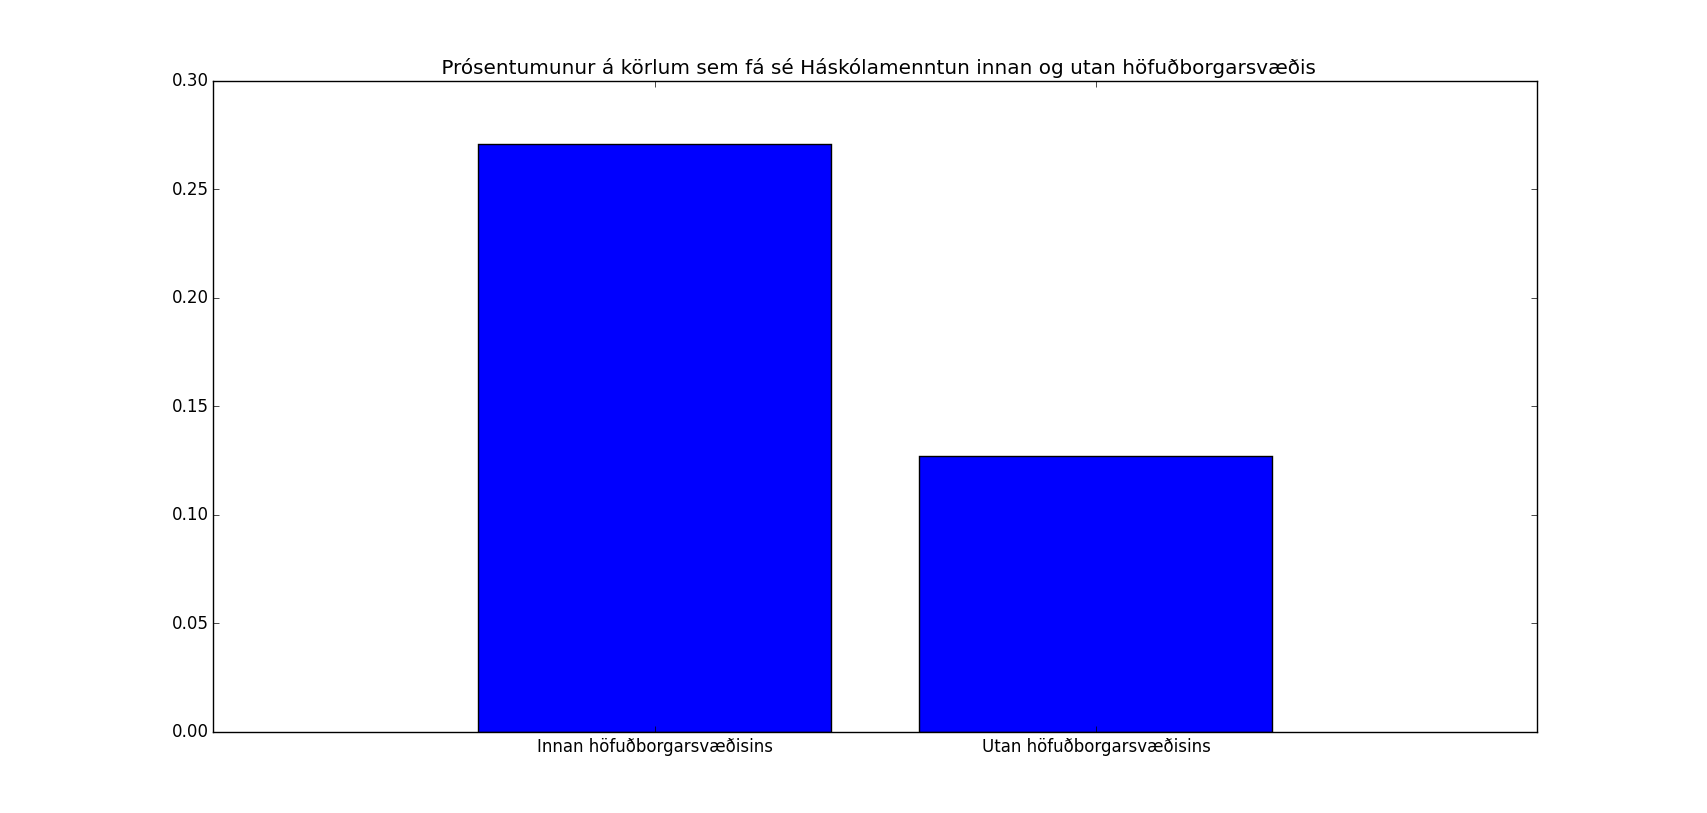
\includegraphics[width=\textwidth]{../graphics/Haskolamentun_karlar_innan_utan_hs.png}
	\caption{Hlutfall karla sem sækja sér háskólamenntun innan og utan höfuðborgarsvæðisins \label{fig:menntukarla}}
\end{figure}

\begin{figure}
	\centering 
	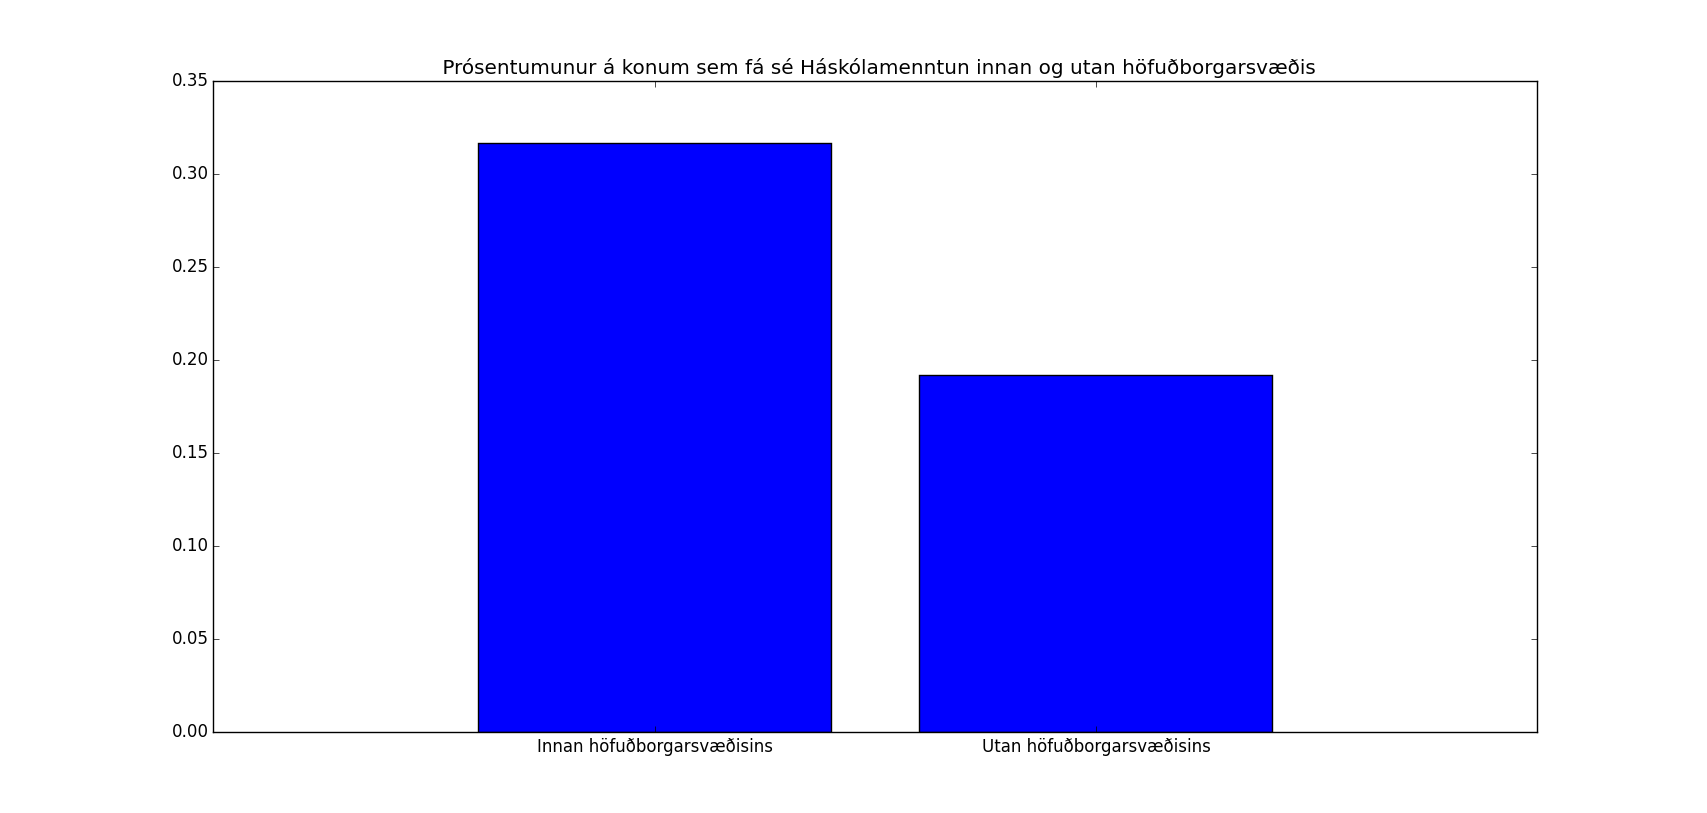
\includegraphics[width=\textwidth]{../graphics/Haskolamentun_konur_innan_utan_hs.png}
	\caption{Hlutfall kvenna sem sækja sér háskólamenntun innan og utan höfuðborgarsvæðisins\label{fig:menntunkonur}}
\end{figure}

\begin{figure}
	\centering 
	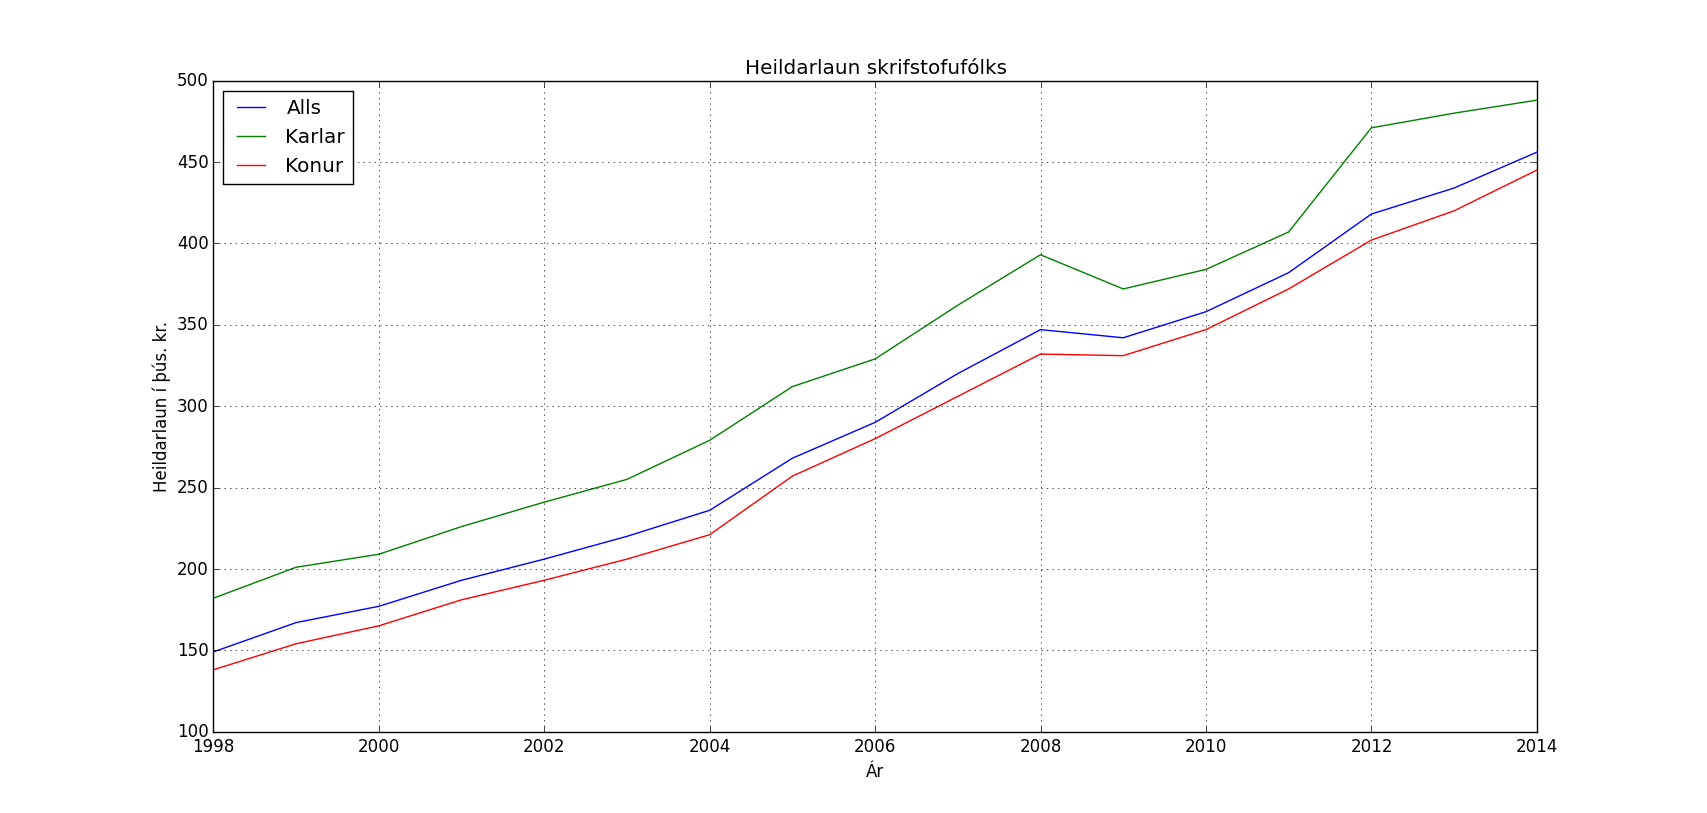
\includegraphics[width=\textwidth]{graphics/heildar_laun.png}
	\caption{Meðaltal heildarlauna karla, kvenna og beggja í skrifstofustarfi \label{fig:heildarlaun}}
\end{figure}

\begin{figure}
	\centering 
	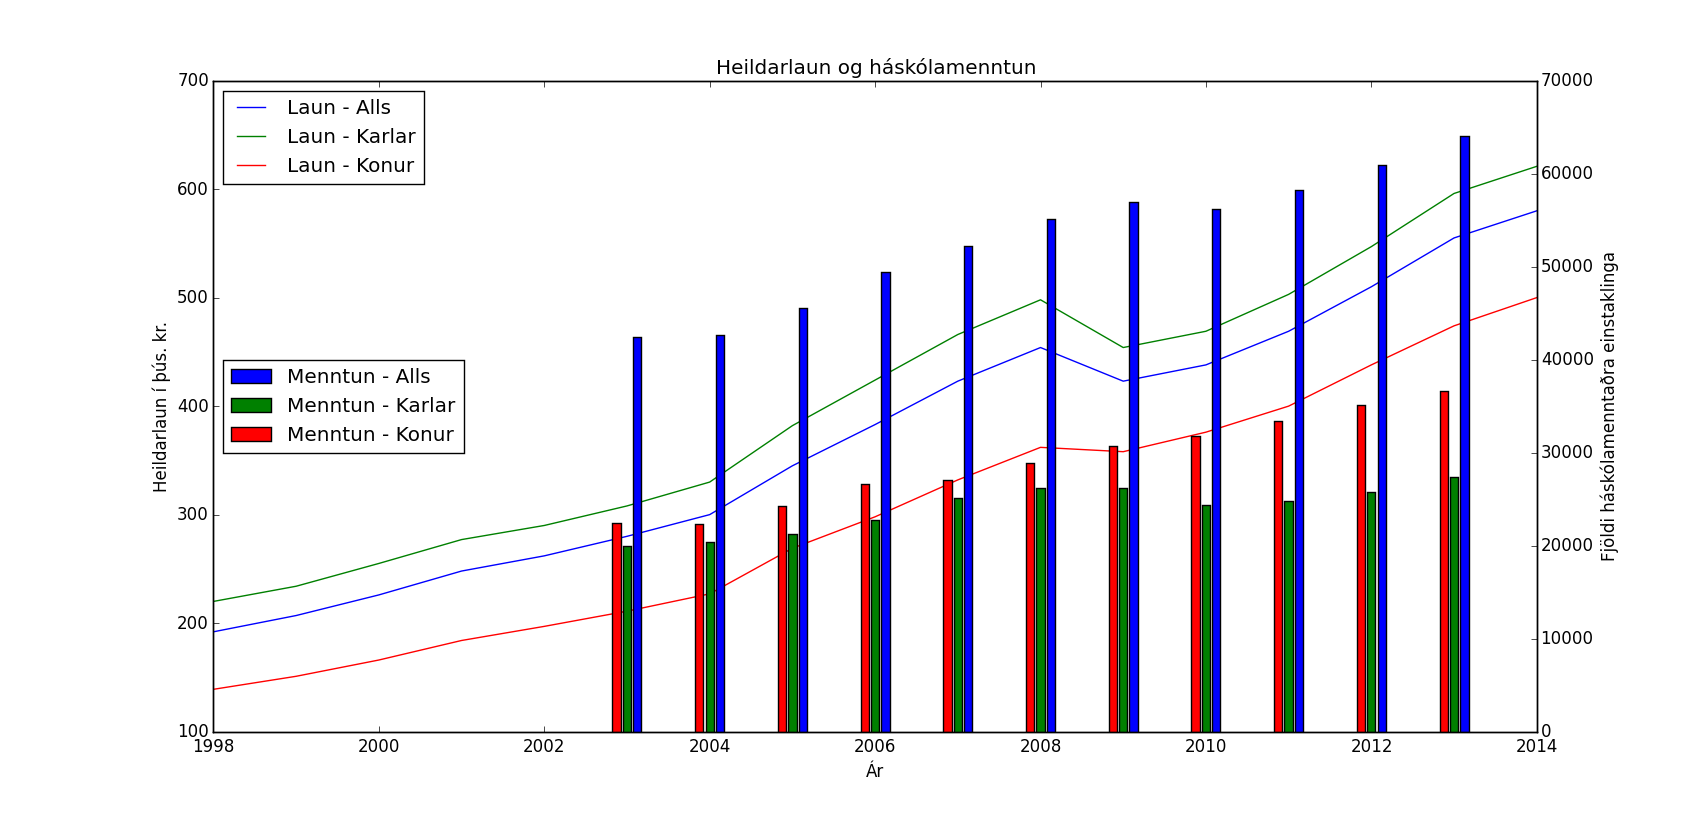
\includegraphics[width=\textwidth]{graphics/heildar_laun_og_haskolamentun.png}
	\caption{Meðaltal heildarlauna karla, kvenna og beggja á vinnumarkaði ásamt háskólamenntun \label{fig:heildarhask}}
\end{figure}

%\begin{figure}
%	\centering 
%	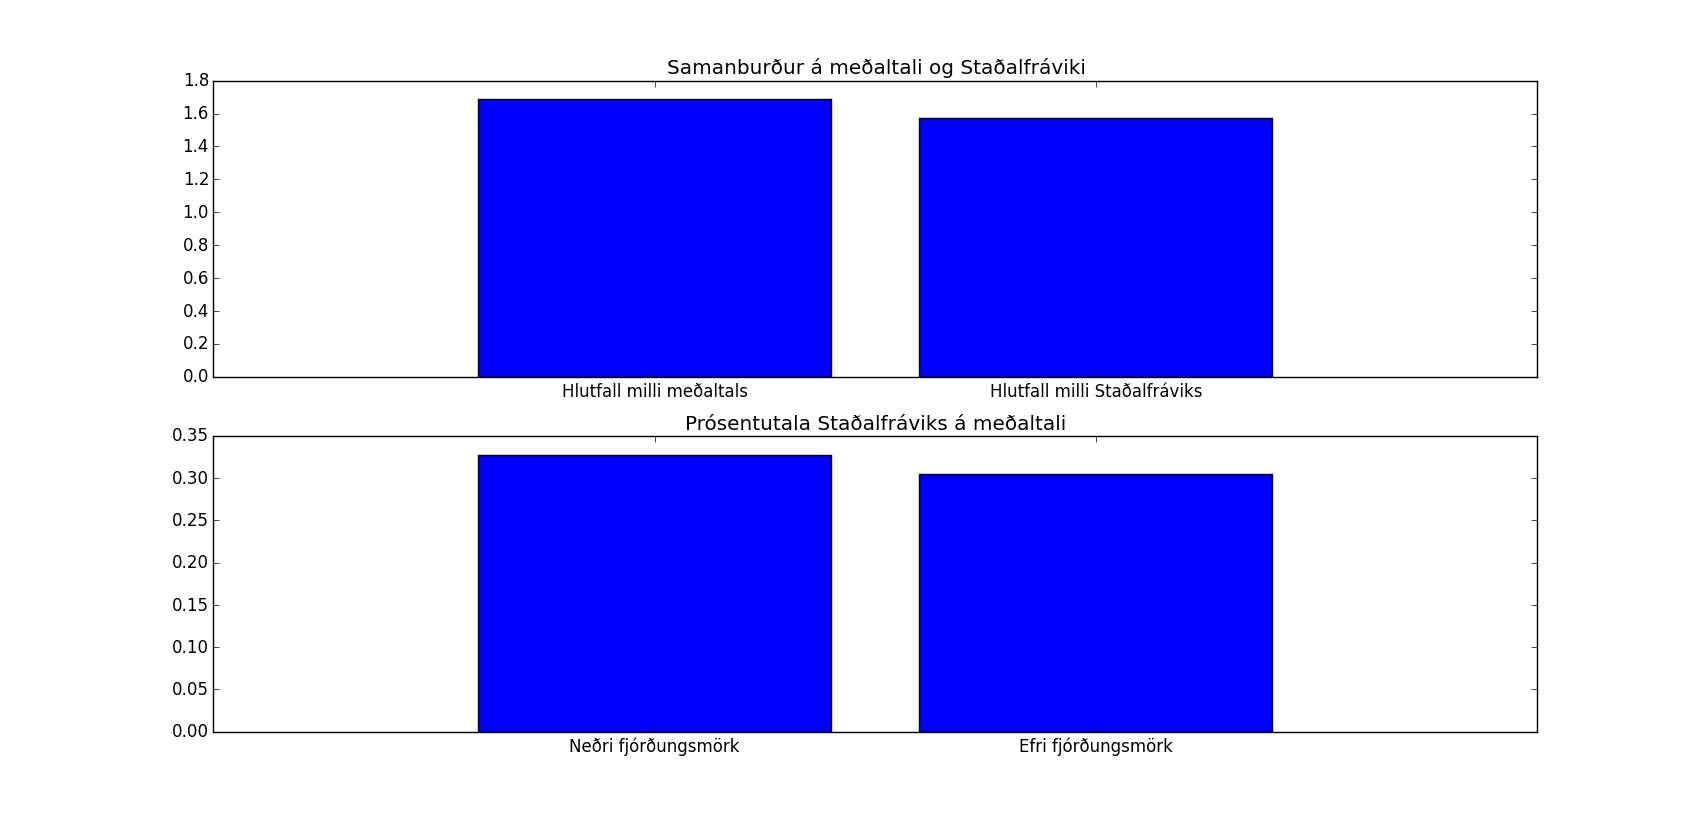
\includegraphics[width=\textwidth]{../graphics/medaltal_stadalfravik_menntun_utan_innan_hs.png}
%	\caption{Meðallaun og staðalfrávik efri og neðri fjórðungsmarka \label{fig:stdhs}}
%\end{figure}

\begin{figure}
	\centering 
	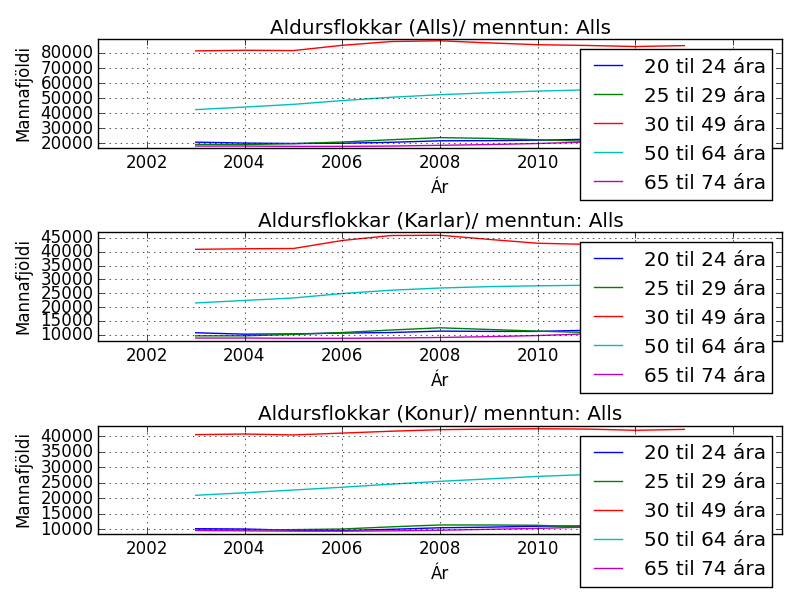
\includegraphics[width=\textwidth]{../graphics/mentun_aldrusflokkar_alls.png}
	\caption{Aldurflokkar / menntun: Alls \label{fig:menntunall}}
\end{figure}

\begin{figure}
	\centering 
	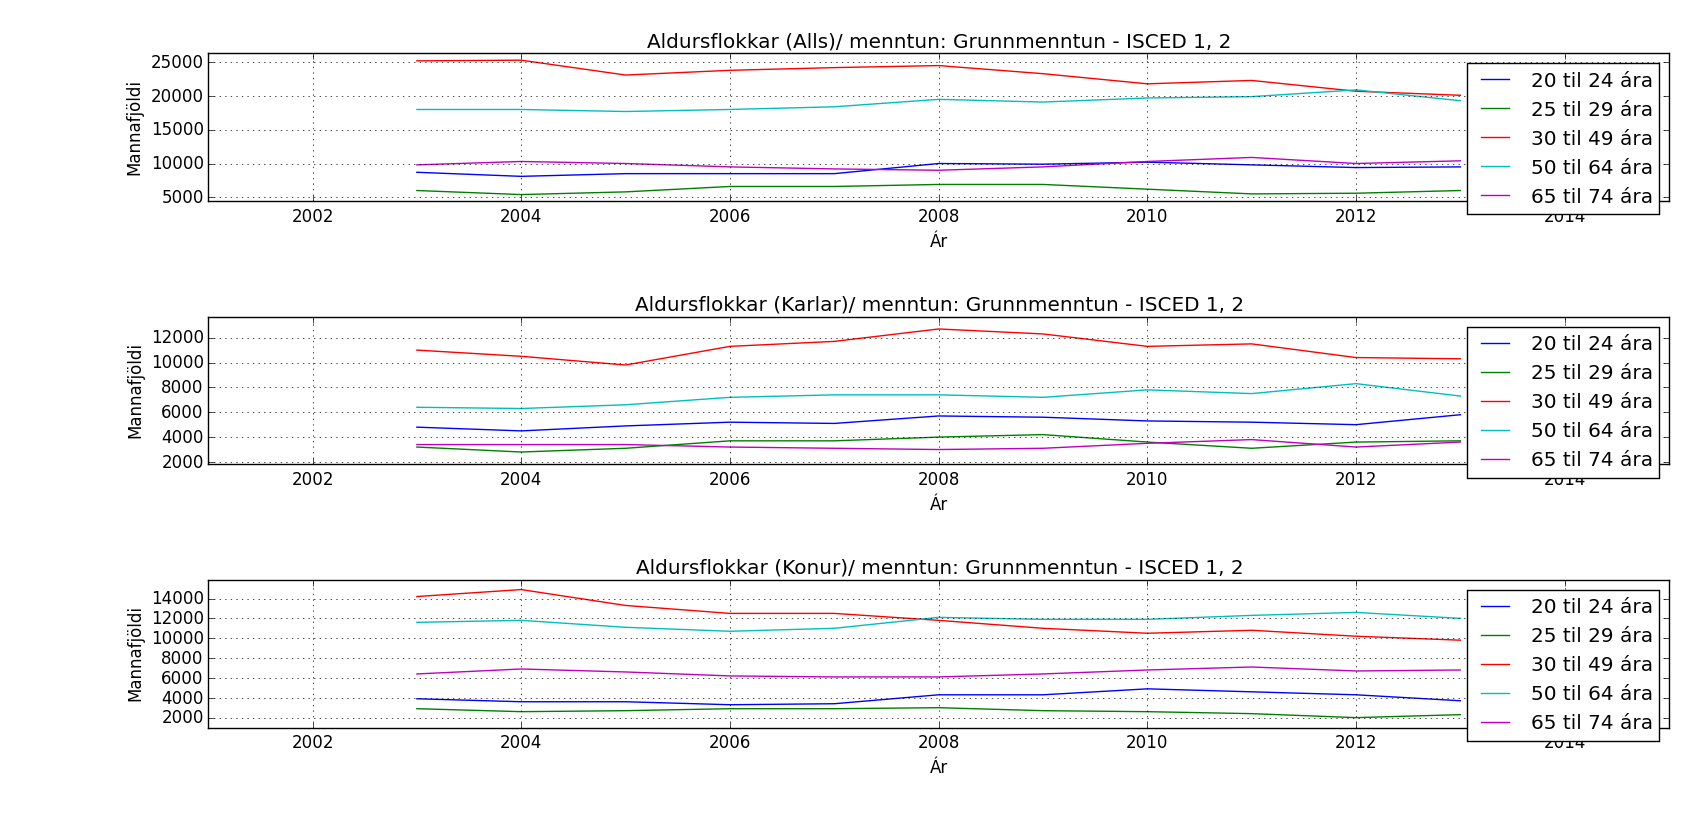
\includegraphics[width=\textwidth]{../graphics/mentun_aldrusflokkar_grunnmenntun.png}
	\caption{Aldurflokkar / menntun: Grunn- \label{fig:menntungrunn}}
\end{figure}

\begin{figure}
	\centering 
	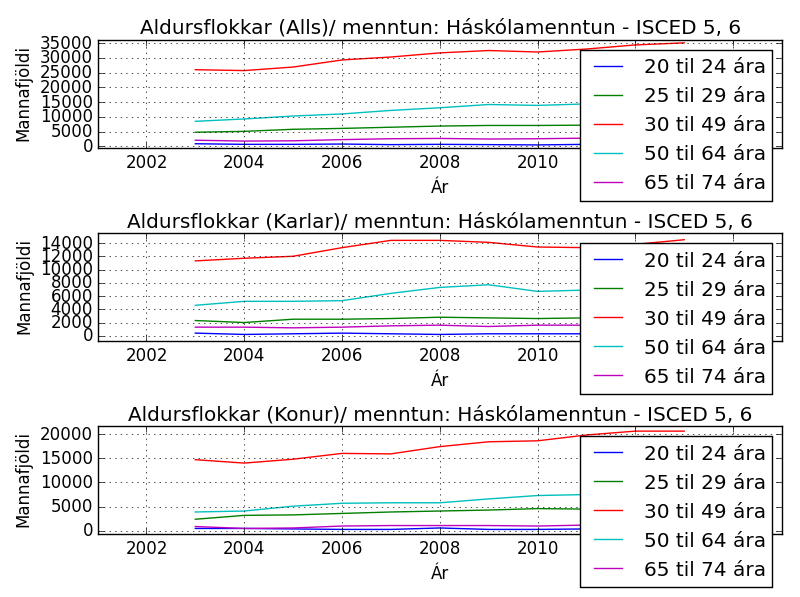
\includegraphics[width=\textwidth]{../graphics/mentun_aldrusflokkar_haskolamenntun.png}
	\caption{Aldurflokkar / menntun: Háskóla- \label{fig:menntunhs}}
\end{figure}

\begin{figure}
	\centering 
	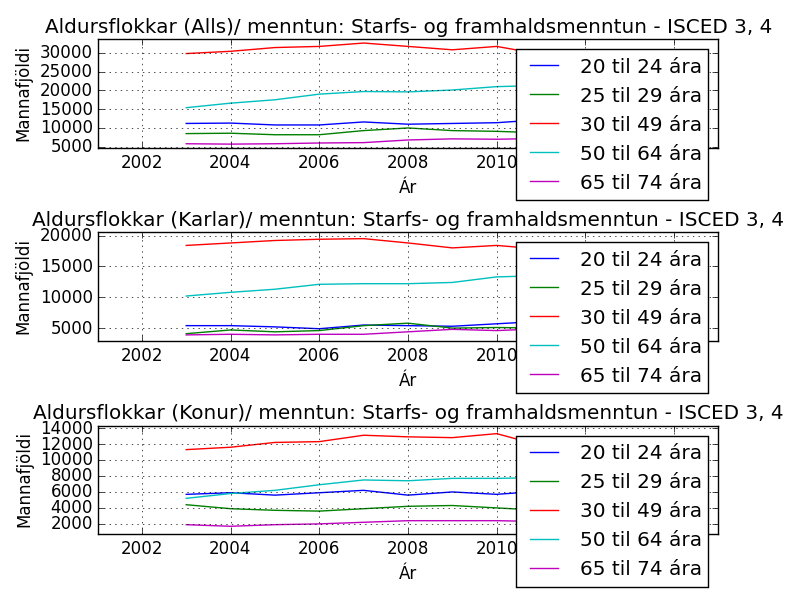
\includegraphics[width=\textwidth]{../graphics/mentun_aldrusflokkar_starfs_og_framhaldsmenntun.png}
	\caption{Aldurflokkar / menntun: Framhalds- Alls \label{fig:menntunfram}}
\end{figure}

\begin{figure}
	\centering 
	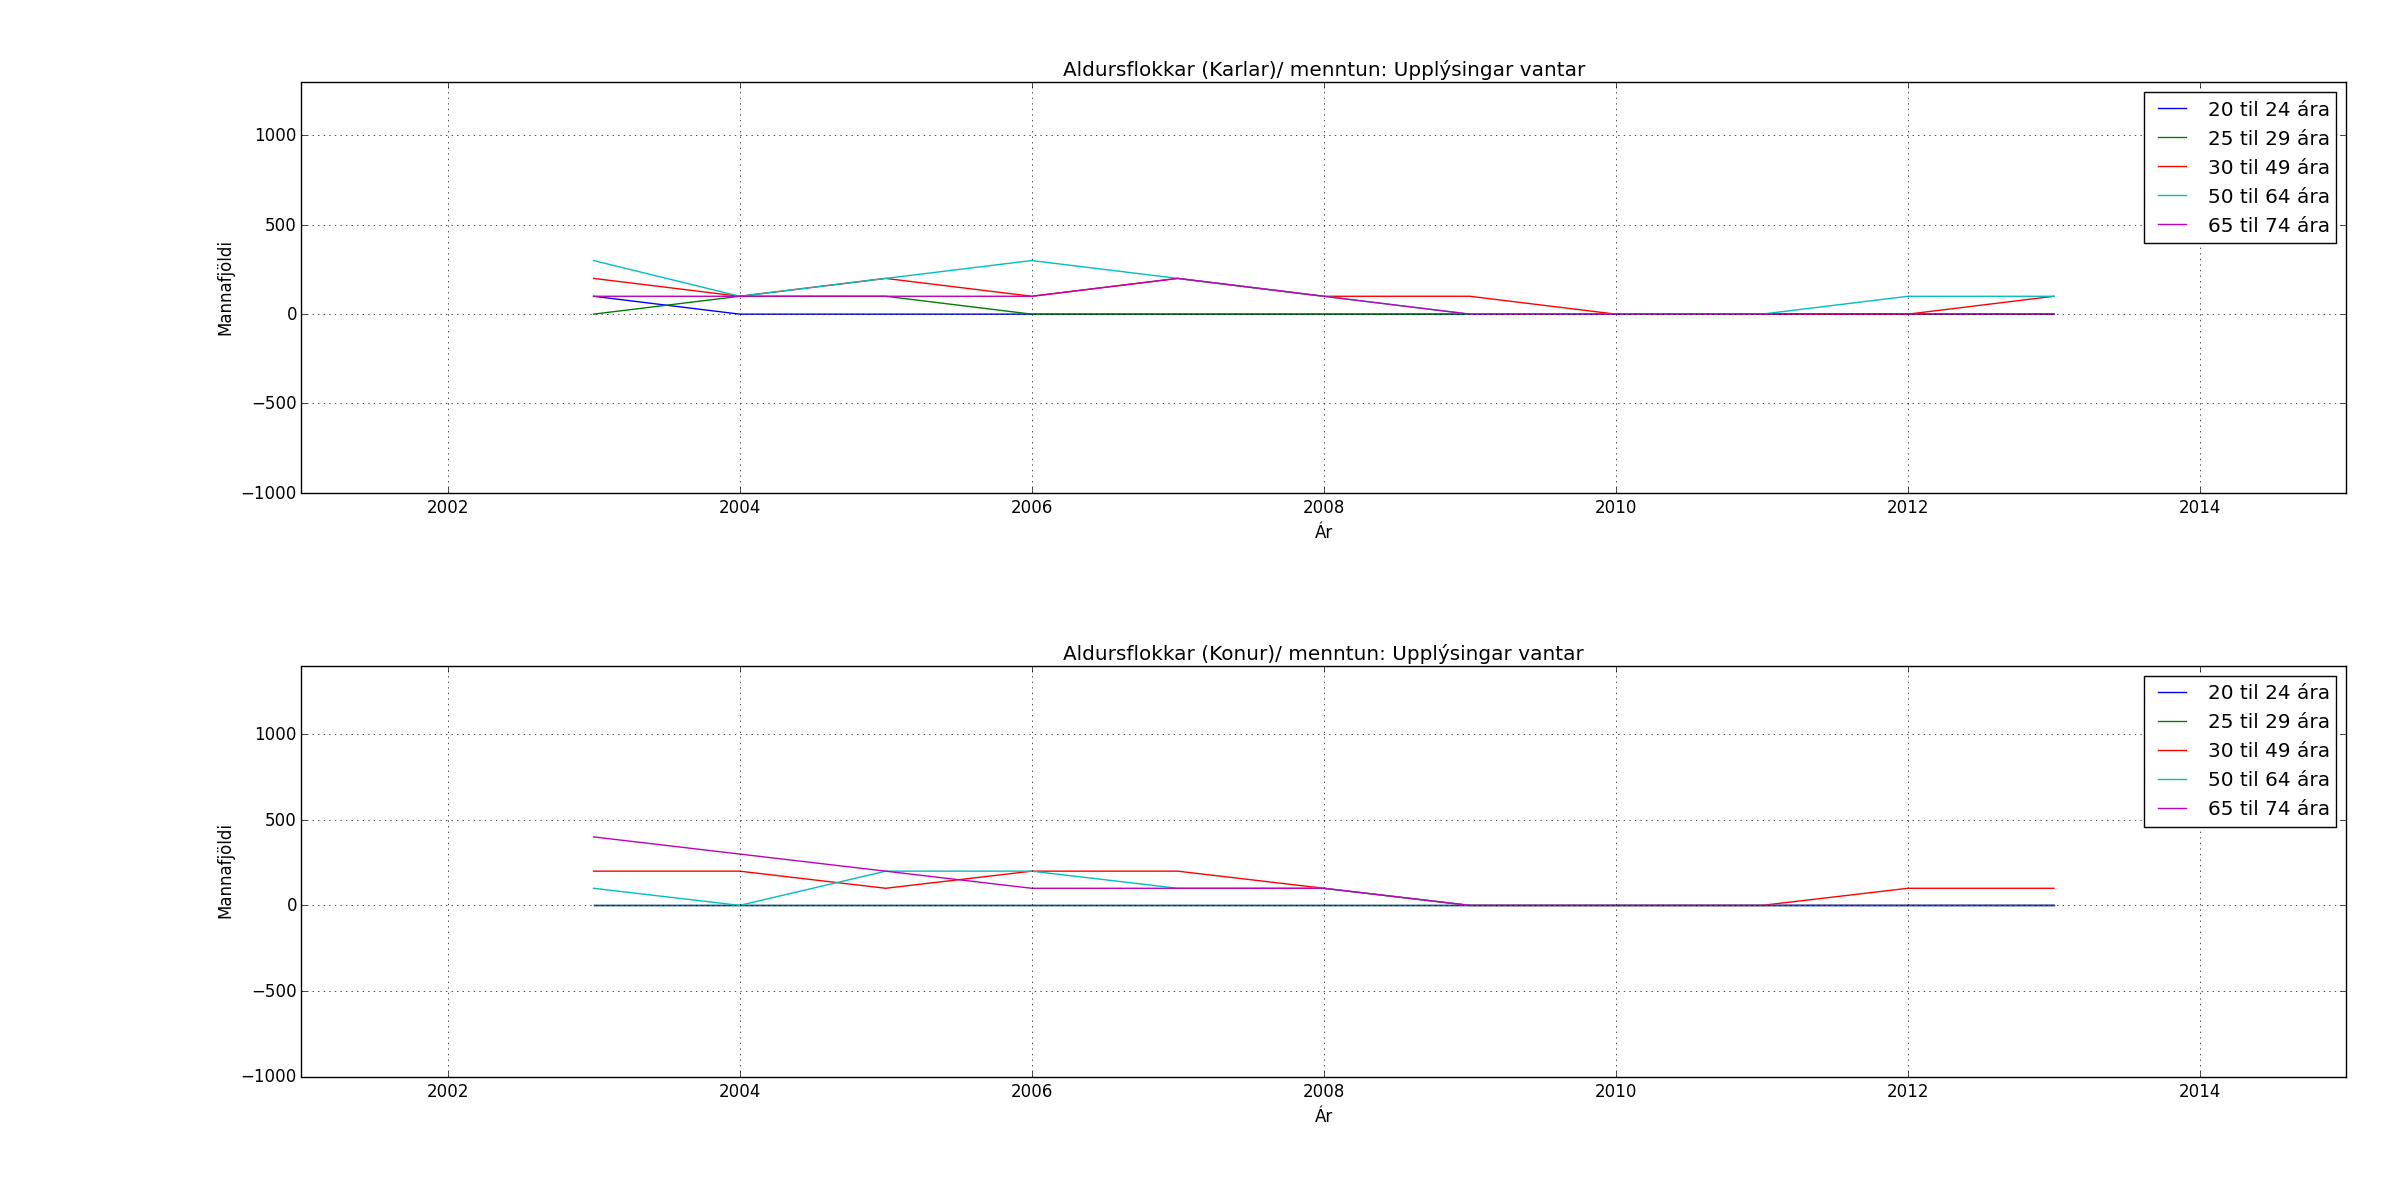
\includegraphics[width=\textwidth]{../graphics/mentun_aldrusflokkar_upplysingar_vantar.png}
	\caption{Aldurflokkar / menntun: Upplýsingar vantar \label{fig:menntunvantar}}
\end{figure}

\begin{figure}
	\centering 
	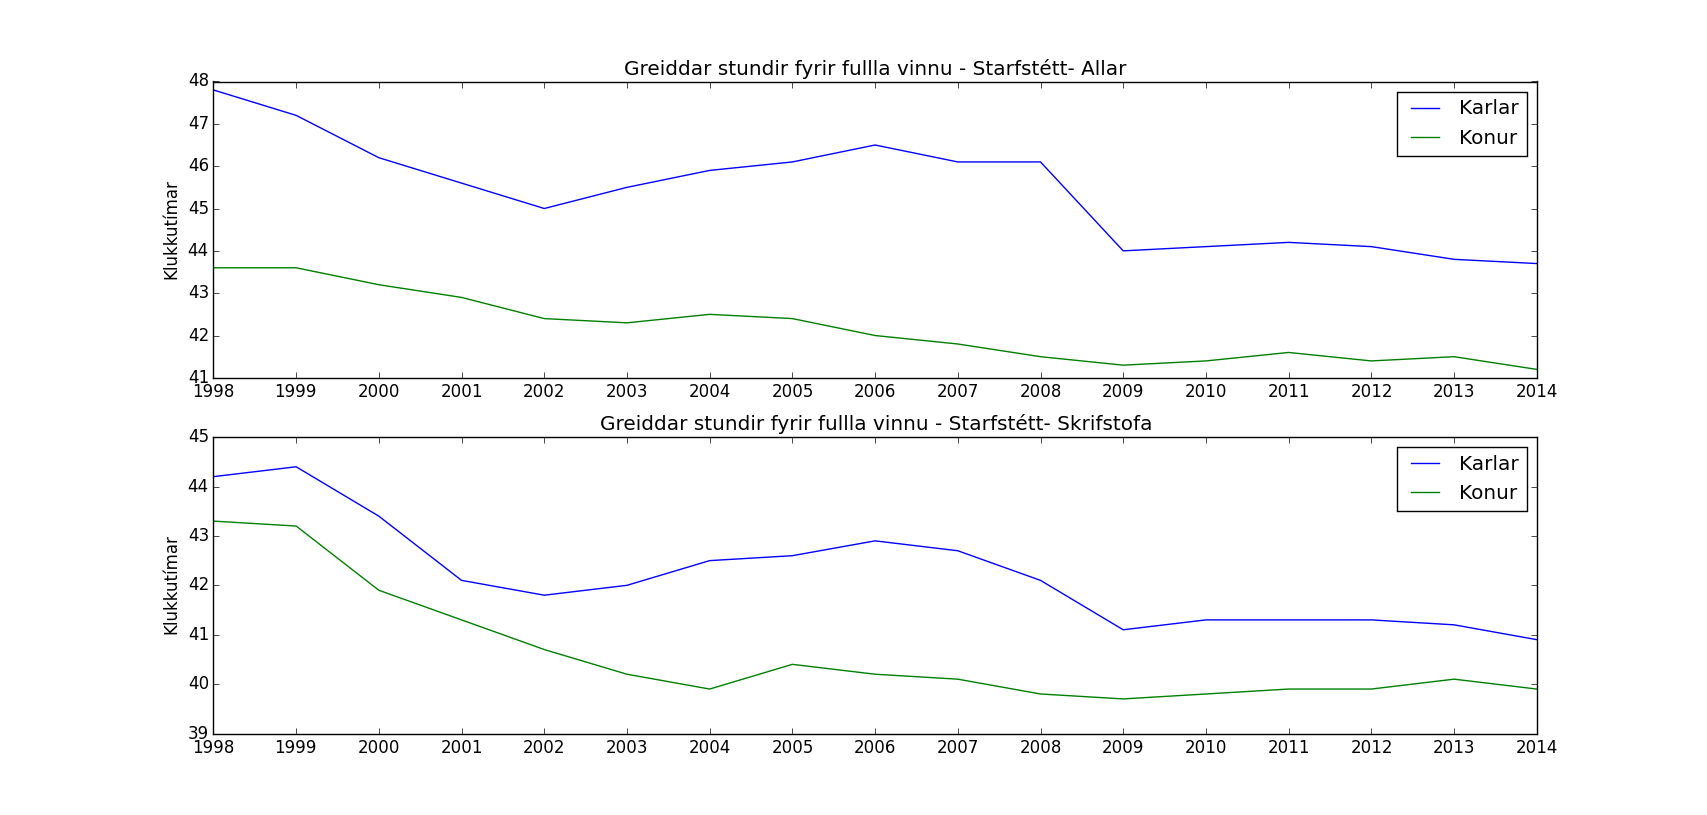
\includegraphics[width=\textwidth]{../graphics/unnir_timar1.png}
	\caption{Greiddar vinnustundir hjá öllum vinnustéttum og skrifstofufólki \label{fig:unnirtimar1}}
\end{figure}

\begin{figure}
	\centering 
	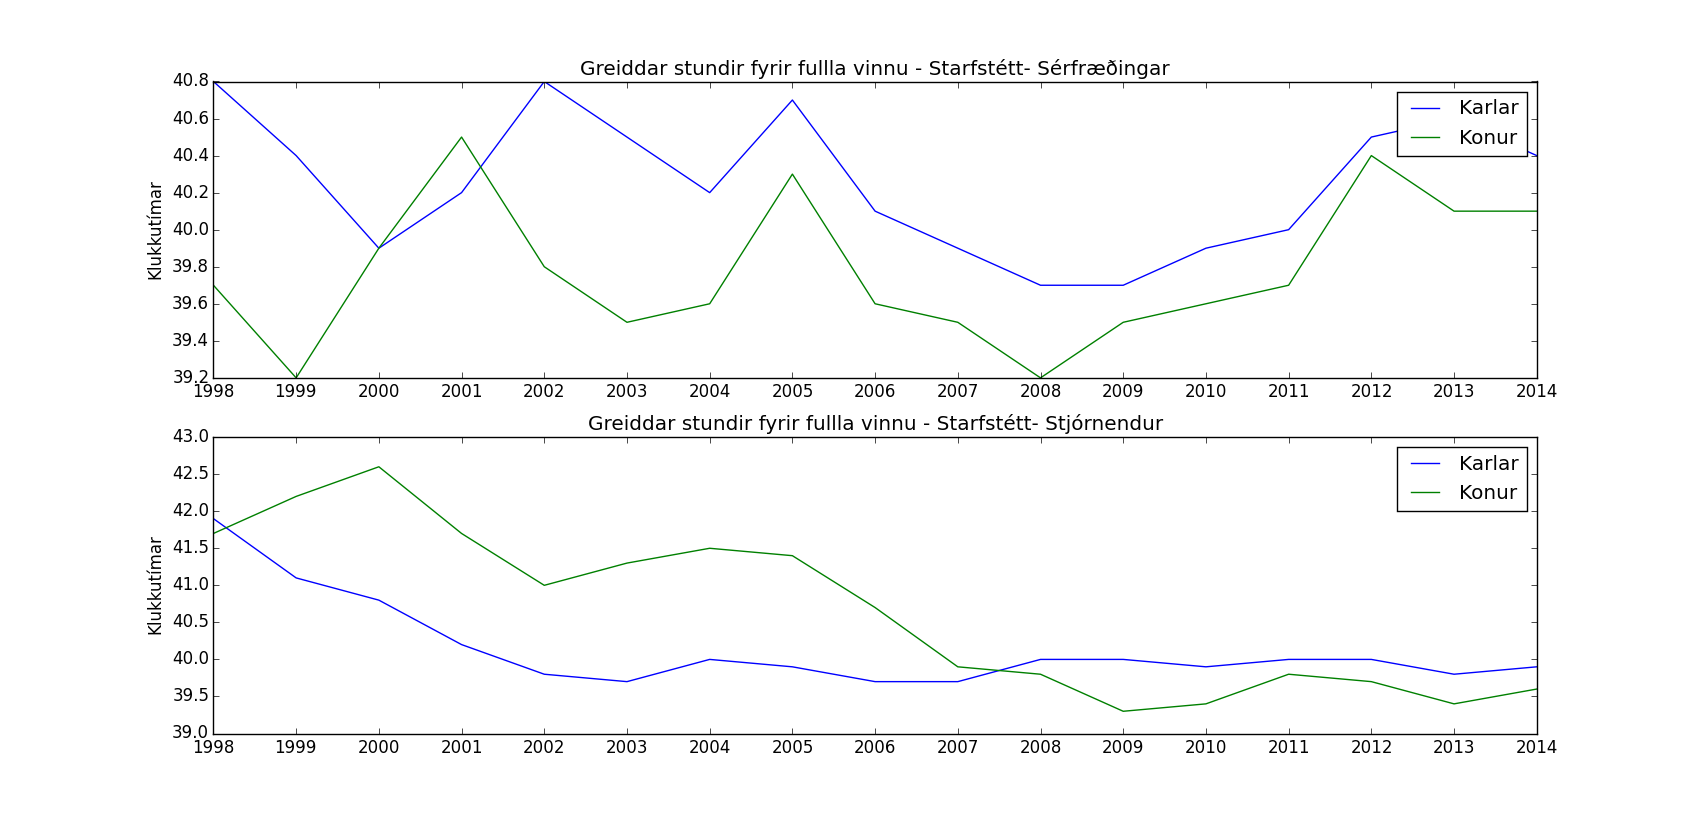
\includegraphics[width=\textwidth]{../graphics/unnir_timar2.png}
	\caption{Greiddar vinnustundir hjá sérfræðimenntuðu fólki og stjórnendum \label{fig:unnirtimar2}}
\end{figure}

\begin{figure}
	\centering
	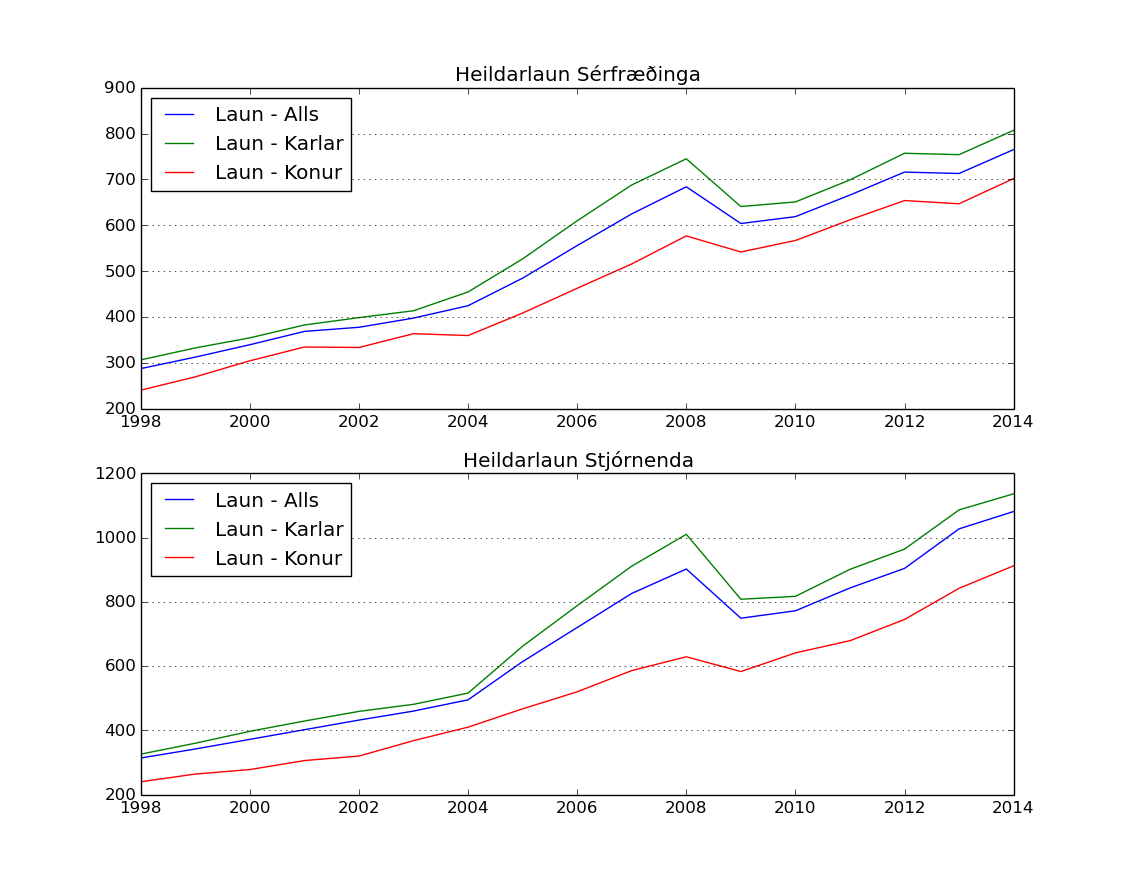
\includegraphics[width=\textwidth]{heildar_laun_stjorn_serfr}
	\caption{Heildarlaun sérfræðimenntaðs fólks og stjórnenda}
	\label{fig:heildarlaunstjorn}
\end{figure}

%
\clearpage
\printbibliography

\end{document} % this tells the compiler that we are done

% These are variables for the editor Emacs
%%% Local Variables: 
%%% TeX-command-BibTeX: biber
%%% mode: latex
%%% TeX-master: t
%%% End:
